%!TEX TS-program = xelatex
%!TEX encoding = UTF-8 Unicode

\documentclass[12pt]{article}
\usepackage{geometry}                % See geometry.pdf to learn the layout options. There are lots.
\geometry{a4paper,top=2cm}
\usepackage[parfill]{parskip}    % Activate to begin paragraphs with an empty line rather than an indent
\usepackage{graphicx}
\usepackage{amsmath}
\usepackage{amssymb}
\usepackage{mathtools}
\usepackage{physics}
\newcommand{\be}{\begin{equation}}
\newcommand{\ee}{\end{equation}}
\usepackage[thicklines]{cancel}
\usepackage{url}
\usepackage{booktabs}
\usepackage{csquotes}
\usepackage{qcircuit}
\usepackage{circledsteps}
\usepackage{nicefrac}
\usepackage{fontspec,xltxtra,xunicode}
\usepackage{xcolor}
\defaultfontfeatures{Mapping=tex-text}

\newcommand{\polv}{\ensuremath{\updownarrow}}
\newcommand{\polh}{\ensuremath{\leftrightarrow}}
\newcommand{\poldr}{\rotatebox[origin=c]{45}{\ensuremath{\leftrightarrow}}}
\newcommand{\poldl}{\rotatebox[origin=c]{-45}{\ensuremath{\leftrightarrow}}}
\newcommand{\bigzero}{\mbox{\normalfont\Large\bfseries 0}}

\title{Advanced Quantum Mechanics\\Class 25}
%\author{The Author}
\date{November 24, 2022}                                           % Activate to display a given date or no date

\begin{document}
\maketitle

\setcounter{section}{6}

\section{Approximation Methods}

Reminder of the system we will consider later:
a system, that is a quantum magnetic moment,
 described by an operator $\hat{\vec{\mu}}$;
and an environment: time-dependent magnetic field
$\vec{B}(t)$, with constant magnitude $B=|\vec{B}|$.

\begin{minipage}{0.6\textwidth}
\setcounter{equation}{77}
Hamiltonian of the system is then
\be
\hat{H}(t)=-\hat{\vec{\mu}} \cdot \vec{B}(t)=-g \underbrace{\frac{q}{2 m c}}_{\text{note the c}} \hat{\vec{J}} \cdot \vec{B}
\ee	
Defining the ``coordinates'' $\vec{R}(t)=B \hat{R}(t)$ and
\be
b=-g \frac{q}{2 m c} B
\ee
one can write $\hat{H}$ as
\be
\hat{H}(t)=\hat{H}(\vec{R}(t)) \equiv \hat{H}(R)=b \hat{R}(t) \cdot \hat{\vec{J}}
\label{eq:g80}
\ee
\end{minipage}%
\begin{minipage}{0.4\textwidth}
\hfill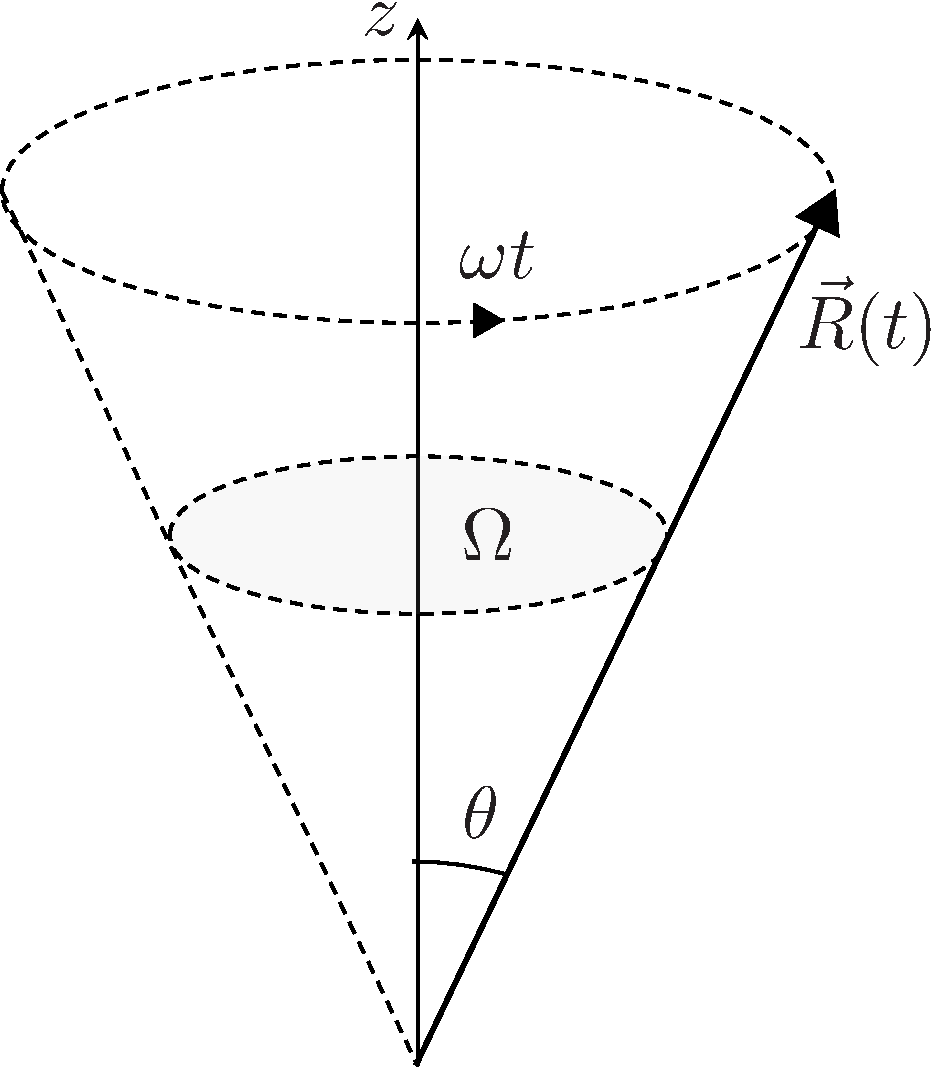
\includegraphics[width=0.9\textwidth]{Figures/RotatingVector-crop.pdf}
\end{minipage}

$\hat{R}(t)$ is a unit vector $\rightarrow$ parameter space of the
environment is \emph{unit sphere}.
An example is the field precessing with
frequency $\omega$ about the $\hat{z}$ direction:
\be
\vec{R}(t)=\hat{x} \sin \theta \cos (\phi+\omega t)+ \hat{y} \sin \theta \sin (\phi+\omega t)+\hat{z} \cos \theta
\label{eq:g81}
\ee
(counter clockwise precession)

\rule{\textwidth}{1pt}

%%%

\setcounter{subsection}{2}
\subsection{Adiabatic approximation (continued)}
\setcounter{equation}{95}

Adiabatic time development:
\be
|\psi(t)\rangle\langle\psi(t)|=| n ; R(t)\rangle\langle n ; R(t)|=P_{n}(R(t))
\label{eq:g96}
\ee
or
\be
\hat{\rho}(t)=P_{n}(R(t))
\ee
a generalization of the condition that
a state is \emph{stationary}, \textit{i.e.}
\be
\hat{\rho}(t)=|\psi(t)\rangle\langle\psi(t)|=| \psi(0)\rangle\langle\psi(0)|
\ee
\emph{But}, it should be clear that Eq.~\eqref{eq:g96} is an
approximation, \textit{i.e.} it cannot be an exact
statement, because:
%%% 05 OKAY
\[
i \hbar \frac{d \hat{\rho}(t)}{d t}=[\hat{H}(R), \hat{\rho}(t)]
\]
which by the adiabatic assumption means
\be
i \hbar \frac{d \hat{\rho}(t)}{d t}=\left[\hat{H}(R), \hat{\rho}_{n}(R)\right]=0
\label{eq:g99}
\ee
which means
\be
\hat{\rho}(t) = \text{ constant } = \hat{\rho}(0)
\ee
and \emph{not} Eq.~\eqref{eq:g96}.

In particular, Eq.~\eqref{eq:g99} means that if
$\hat{\rho}(t)=P_{n}(t)$, the motion of the system cannot
be cyclic (or periodic), \textit{i.e.} $\hat{\rho}(0) \neq \hat{\rho}(T)$, where
$T$ is the time to come back to the same state.

\emph{Conclusions:}
\begin{enumerate}
\item \emph{exact} adiabatic cyclic evolutions do not exist
\item adiabaticity can only be an approximation
\end{enumerate}

\setcounter{subsubsection}{2}
\subsubsection{Validity of the adiabatic approximation}

\begin{quote}\emph{Skipped in class, jump straight to Eq.~\eqref{eq:g103}}\end{quote}

Let as write $\ket{\psi(t)}$ in the basis $\{|n ; R(t)\rangle\}$:
%%% 06 OKAY
\be
|\psi(t)\rangle=\sum_{m} C_{m}(t)|m ; R(t)\rangle
\label{eq:g101}
\ee
and suppose $|\psi(0)\rangle=|n, R(0)\rangle$. Therefore, the
adiabatic approximation is valid \textit{only if} one
can ignore all $C_m(t)$ in \eqref{eq:g101}, with the exception
of $m=n$:
\be
|\psi(t)\rangle=C_{n}(t)|n ; R(t)\rangle
\ee
where $C_n(0)=1$, because $|\psi(0)\rangle=|n, R(0)\rangle$.
Use this $|\psi(t)\rangle$ in Schrödinger equation:% \eqref{eq:g82}:
\[
\left(i \hbar \frac{d}{d t} C_{n}(t)\right)
|n ; R(t)\rangle+i \hbar C_{n}(t) \frac{d}{d t}|n ; R(t)\rangle=
C_{n}(t) \underbrace{\hat{H}|n ; R\rangle}%
_{E_n(R)\ket{n,R}}
\]
Project this onto $|m ; R\rangle, m \neq n$,
leading to\\
\rule{\textwidth}{1pt}
\be
\left\langle m ; R(t) \mid \frac{d}{d t} \mid n ; R(t)\right\rangle=0, \quad m \neq n
\label{eq:g103}
\ee
that is the condition for validity of the adiabatic approximation.

Note that the scalar product in Eq.~\eqref{eq:g103}, when
referring to a problem in ordinary space where
the coordinates of the system are denoted by $\vec{r}$,
is given by
%%% 07 OKAY
\be
\left\langle m ; R(t)\left|\frac{d}{d t}\right| n ; R(t)\right\rangle=\int d^{3} r\, \psi_{m}^{*}(\vec{r}, R(t)) \frac{d}{d t} \psi_{n}(\vec{r}, R(t))
\ee
$\rightarrow$
important not to confuse the
coordinates of the environment, $\vec{R}(t)$,
with the ordinary coordinates $\vec{r}$.

\begin{quote}\emph{Skipped in class, jump straight to Eq.~\eqref{eq:g108}}\end{quote}

One can reexpress  Eq.~\eqref{eq:g103} in terms of the derivative
of the Hamiltonian $\hat{H}(R(t))$ w.r.t. the time:
\begin{enumerate}
\item let us start differentiating the eigenvalue
equation:
\[
\begin{gathered}
\hat{H}(R)|n ; R\rangle=E_{n}(R)|n ; R\rangle\\
\langle m ; R \mid n ; R\rangle=\delta_{m n}
\end{gathered}
\] 
so:
\be
\begin{gathered}
\left(\frac{d \hat{H}(R(t))}{d t}\right)|n ; R(t)\rangle+\hat{H}(R(t)) \frac{d}{d t}|n ; R(t)\rangle= \\ 
\frac{d E_{n}(R(t))}{d t}\left|n ; R(t)\right\rangle+E_{n}(R(t)) \frac{d}{d t}|n ; R(t)\rangle
\end{gathered}
\ee
%
\item project this out $\ket{m;R(t)}$, with $ m\neq m$:
\be
\begin{gathered}
\left\langle m ; R\left|\frac{d}{d t} \hat{H}\right| n ; R\right\rangle+E_{m}(R)\left\langle m ; R\right| \frac{d}{d t}\left| n ; R\right\rangle \\ 
=E_{n}(R)\langle m ; R| \frac{d}{d t}|n ; R\rangle, m \neq n 
\end{gathered}
\ee
%%%% 08
\item This then leads immediately to:
\be
\underbrace{\left\langle m ; R\left|\frac{d}{d t}\right| n ; R\right\rangle}%
_{=0\text{ by Eq.~\eqref{eq:g103}}}
=\frac{\langle m ; R|d \hat{H} / d t| n ; R\rangle}{E_{n}(R)-E_{m}(R)},\,m \neq n
\ee
%
\item This implies:\\
\rule{\textwidth}{1pt}
\be
\frac{\langle m ; R|d \hat{H} / d t| n ; R\rangle}{E_{n}(R)-E_{m}(R)} = 0,\,m \neq n
\label{eq:g108}
\ee
where we see the appearance of $d \hat{H} / d t$ $\rightarrow$ reason for the name ``adiabatic''.
\end{enumerate}

\subsubsection{Berry's phase}

Suppose $|\psi(0)\rangle=|n ; R(0)\rangle$ and that the adiabatic
approximation is valid; then
\be
|\psi(t)\rangle=\sum_m C_{m}(t)|m ; R(t)\rangle=C_{n}(t)|n ; R(t)\rangle
\ee
with $C_n(0) = 1$.
Using this into the Schrödinger equation:
%%% 09
\be
\begin{aligned}
i \hbar \frac{d}{d t}|\psi(t)\rangle
&=i \hbar \frac{d C_{n}(t)}{d t}|n ; R(t)\rangle+i \hbar C_{n} (t) \frac{d}{d t}|n ; R(t)\rangle\\
&=E_{n}(R(t)) C_{n}(t)\left|n ; R(t)\right\rangle
\end{aligned}
\ee
Projecting onto $\ket{n;R(t)}$:
\be
\frac{d C_{n}(t)}{d t}=-C_{n}(t)
\left[i / \hbar E_{n}(t)+\langle n ; R(t)|\frac{d}{d t}|n ; R(t)\rangle\right]
\label{eq:g111} 
\ee
Taking into account the initial condition $C_{n}(0)=1$, the
integration of \eqref{eq:g111} leads to:
\be
C_{n}(t)=e^{-i / \hbar \int_{0}^{t} d t^{\prime} E_{n}\left(t^{\prime}\right)} e^{i \gamma_{n}(t)}
\ee
where the phase angle $\gamma_n(t)$ is given by
\be
\gamma_{n}(t)=i \int_{0}^{t} d t^{\prime}\langle n ; R(t^{\prime})|\frac{d}{d t^{\prime}}|n ; R(t^{\prime})\rangle
\ee
Therefore, in the adiabatic approximation:
\be
\ket{\psi(t)} = e^{-i / \hbar \int_{0}^{t} d t^{\prime} E_{n}\left(t^{\prime}\right)} e^{i \gamma_{n}(t)} \ket{n;R(t)}
\ee
where the first phase is the \emph{dynamical phase}, 
and the second one is the \emph{geometric phase}.

%%% 10
$\gamma_{n}(t)$ has a striking property: it does not depend
on the time dependence of the integrand; it depends 
on the path $\vec{R}(0) \to \vec{R}(t)$  in parameter space.
\be
\frac{d}{d t^{\prime}}\left|n ; R\left(t^{\prime}\right)\right\rangle d t^{\prime}=\frac{\partial}{\partial R_{i}\left(t^{\prime}\right)}\left|n ; R\left(t^{\prime}\right)\right\rangle d R_{i}\left(t^{\prime}\right)
\ee
so
\begin{align}
\gamma_{n}(t)
&=i \int_{R(0)}^{R(t)} d R_{i}\langle n ; R| \frac{\partial}{\partial R_{i}}\left|n ; R\right\rangle\nonumber\\
&=i \int_{R(0)}^{R(t)} d \vec{R} \cdot\left\langle n ; R\left|\vec{\nabla}_{\!R}\right| n ; R\right\rangle\\
&=i \int_{C} d \vec{R} \cdot \vec{A}_{n}(R)
\end{align}
where $C$ denotes the curve $C$ that extends from
$\vec{R}(0)$ to $\vec{R}(t)$, and $\vec{A}_{n}(R)$ is the ``vector
potential'':
\be
\vec{A}_{n}(R)=i\langle n ; R|\vec{\nabla}_{\!R}| n ; R\rangle
\label{eq:g118}
\ee
Can one get rid of such a phase? Yes, almost always:
%%% 11 OKAY
\begin{enumerate}
\item The eigenstates of $\hat{H}(R)$ are defined up to
a phase. Therefore, under a gauge transformation:
%Eq.~\eqref{eq:g89}:
\be
\begin{aligned}
|n ; R\rangle \rightarrow|n ; R\rangle^{\prime} 
&=e^{i \phi_{n}(R)}|n ; R\rangle \\
A_{n}(R) \rightarrow A_{n}^{\prime}(R) 
&=i\langle n ; R| \vec{\nabla}_{\!R} |n ; R\rangle^{\prime} \\ 
&=i\langle n ; R| e^{-i \phi_{n}(R)} \vec{\nabla}_{\!R}  e^{i \phi_{n}(R)}|n ; R\rangle\\ 
&=\vec{A}_{n}(R)-\vec{\nabla}_{\!R}  \phi(R) 
\end{aligned}
\ee
%
\item Under such a transformation, the phase angle $\gamma_{n}(t)$
transforms as
\be
\begin{aligned} 
\gamma_{n}(t) \rightarrow \gamma_{n}^{\prime}(t) 
&=\int_{R(0)}^{R(t)} d \vec{R} \cdot \vec{A}_{n}^{\prime}(R) \\ 
&=\gamma_{n}(t)-\int_{R(0)}^{R(t)} d \vec{R} \cdot \vec{\nabla}_{\!R}  \phi_{n}(R) \\
&=\gamma_{n}(t)-\phi_{n}(R(t))+\phi_{n}(R(0))
\end{aligned}
\ee
%
\item Therefore, had the initial condition being
taken $|n, R\rangle^{\prime}$, one would have obtained:
\be
\begin{aligned} 
|\psi_{n}(t)\rangle
&=e^{-i / \hbar \int_{0}^{t} d t^{\prime} E_{n}\left(t^{\prime}\right)} e^{i \gamma_{n}^{\prime}(t)}|n, R(t)\rangle^{\prime}\\
%%% 12 OKAY
&=e^{-i / \hbar \int_{0}^{t} d t^{\prime} E_{n}\left(t^{\prime}\right)} e^{i \gamma_{n}^{\prime}(t)}e^{i\phi_n(R)}|n, R(t)\rangle
\end{aligned} 
\ee
%
\item Since $\phi_{n}(R)$ is arbitrary, one can choose it
to cancel $\gamma_{n}^{\prime}(t)$, \textit{i.e.}
\be
\phi_{n}(R)=-\gamma_{n}^{\prime}(R)
\ee
or, equivalently:
\be
\begin{gathered}
\cancel{\phi_{n}(R)}=-\gamma_{n}(R)+\cancel{\phi_{n}(R)}-\phi_{n}(R(0))\\
\Rightarrow \phi_{n}(R(0))=-\gamma_{n}(R)
\end{gathered}
\ee
%
\item In the above we used the fact that
$\phi_{n}(R(t))$ was arbitrary. \emph{But}, if after some
time $T$ the environmental parameters return to
their original values:
\be
R(0) \rightarrow R(t) \rightarrow R(T)=R(0)
\label{eq:g124}
\ee
then one \emph{cannot} choose $\phi_{n}(R(t))$ freely to
remove $\gamma_{n}(T)$, because $\gamma_{n}(t)$ does not change
under \eqref{eq:g124} : from Stokes' theorem, one has
%%% 13 
\be
\gamma_{n}(t)=\oint_{C} d \vec{R} \cdot \vec{A}_{n}(R)=\int_{S} d \vec{s} \cdot\left(\vec{\nabla}_{\!R}  \times \vec{A}_{n}(R)\right)
\label{eq:g125}
\ee
where 
$C$ is the closed curve from the
evolution $\vec{R}(0)=\vec{R}(T)$
and
$S$ is the surface enclosed
by $C$ during evolution.
So, under the above gauge transformation:
\be
\begin{aligned}
\gamma_{n}^{\prime}(t)
&=\int_{S} d \vec{s} \cdot\left(\vec{\nabla}_{\!R}  \times \vec{A}_{n}^{\prime}(R)\right)\\
&=\gamma_{n}(t)-\int_{S} d \vec{s} \cdot
\cancelto{0}{\left[\vec{\nabla}_{\!R}  \times\left(\vec{\nabla}_{\!R}  \phi_{n}(R)\right)\right]}
\end{aligned}
\ee
\end{enumerate}
Therefore, $\gamma_{n}(t)$ is gauge invariant for a
periodic adiabatic motion; no observable can
depend on a gauge choice. So
\emph{$\gamma_n(t)$ is an observable!}

Further insight can be gained by noting that
Eq.~\eqref{eq:g125} can be written in terms of a ``magnetic''
field:
\begin{gather}
\gamma_{n}(R)=\int_{s} d \vec{s} \cdot \underbrace{\left(\vec{\nabla_{\!R}} \times \vec{A}_{n}(R)\right)}=\int_{s} d \vec{s} \cdot \vec{B}_{n}(R)\\
\vec{B}_n(R)
\end{gather}
%%% We skip the whole "slow and fast hamiltonian"
%%% And go directly to the example.

%%% 20
\setcounter{equation}{143}

\emph{Example:} spin-1/2 particle in magnetic field
precessing around $\hat{z}$ (see beginning of the class):
\[
\vec{R}(t)=\hat{x} \sin \theta \cos (\phi+\omega t)+ \hat{y} \sin \theta \sin (\phi+\omega t)+\hat{z} \cos \theta
\]
The Hamiltonian is given by
\[
\hat{H}(t)=\hat{H}(\vec{R}(t)) \equiv \hat{H}(R)=b \hat{R}(t) \cdot \hat{\vec{J}}
\]
so
\be
\hat{H}(t) = 
\frac{b\hbar}{2}
\begin{pmatrix}
 \cos\theta & \sin\theta e^{-i\phi(t)}\\
\sin\theta e^{ i\phi(t)} & -\cos\theta
\end{pmatrix},\,
\phi(t) = \phi+\omega t
\ee
The eigenvalues are $\pm b \hbar / 2$; when $b=0$, there is
degeneracy. The eigenvectors are
\[
\ket{+,\vec{R}} = \begin{pmatrix} \cos(\theta/2)\\\sin(\theta/2)e^{ i\phi(t)}\end{pmatrix},\quad
\ket{-,\vec{R}} = \begin{pmatrix} -\sin(\theta/2)\\\cos(\theta/2)e^{ i\phi(t)}\end{pmatrix}
\]
The calculation of $\vec{B}_+$ or $\vec{B}_-$ is straightforward, but a bit tedious, from Eq.~\eqref{eq:g118}.
Suffice to say that it can be shown that one can write:
\[
\vec{B}_{n}(\vec{R})=-\Im \sum_{m \neq n} \frac{\left\langle m ; R\left|\left[\vec{\nabla}_{R} \hat{H}(R)\right]\right| n ; R\right\rangle \times\left\langle n ; R\left|\left[\vec{\nabla}_{R} \hat{H}(R)\right]\right| m ; R\right\rangle}{\left(E_{n}(R)-E_{n}(R)\right)^{2}}
\]
so the key is to calculate
\be
\vec{\nabla}_{\!R}  \hat{H}(R)=\frac{b \hbar}{2 B} \vec{\sigma}
\ee
and one can write:
\be
\begin{aligned}
\vec{B}_{\pm}(R)
&=-\frac{(b \hbar / 2 B)^{2}}{(b \hbar)^{2}} 
\underbrace{\Im \langle\mp, R|\vec{\sigma}| \pm, R \rangle \times
    \langle\pm, R|\vec{\sigma}| \mp, R \rangle}%
    _{\pm 2\hat{R}\to\text{ Exercise}}\\
&=\mp \frac{(b \hbar / 2 B)^{2}}{(b \hbar)^{2}} 2 \hat{R}\\
&=\mp \frac{\hat{R}}{2 B^{2}}=\mp \frac{\hat{R}}{2 R^{2}}
\end{aligned}
\ee
where we can see the appearance of a ``magnetic monopole'' of strength $1 / 2$ located at the
origin (at the place of degeneracy).
%%% 21 OKAY
The Berry phase in this case is given by:
\be
\gamma_{+}(R)=\int_{S} d \vec{s} \cdot \vec{B}_{+}(R)=-\frac{1}{2 R^{2}} \int_{S} d \vec{s} \cdot \hat{R}
\ee

\begin{minipage}{0.4\textwidth}
Easier to compute:
-- flux through $S$
enclosed by $C$ is the
same is through on $S^{\prime}$
with solid angle $\Omega: d \vec{s}=R^{2} d \Omega \hat{R}$
\end{minipage}%
\hfill
\begin{minipage}{0.6\textwidth}
\[
\begin{cases}
\begin{aligned}
&\text{Closed path $C$: for a given $\theta$, the}\\
&\text{path is from $\theta, \phi$ to $\theta, \phi+2 \pi$ (period).}\\
\end{aligned}
\end{cases}
\]
\vspace{1em}
\end{minipage}

\be
\begin{aligned}
\gamma_{+}(R)
&=-\frac{1}{2 R^{2}} \int R^{2} d \Omega=-\frac{1}{2 R^{2}} \int_{0}^{\theta} d \theta \sin \theta \int_{\phi}^{\phi+2 \pi} d \phi\\
&=-\frac{1}{2}(1-\cos \theta) 2 \pi=-\pi(1-\cos \theta)
\end{aligned}
\ee
We could have used opposite direction of $C$:
\[
\gamma_{\pm}(R)=\mp \frac{1}{2} \Omega, \quad \Omega=2 \pi(1-\cos \theta)
\]
where $\Omega$ is the
solid angle subtended by the
closed path as viewed by
the monopole (origin of the
parameter space).

\emph{Experiment}: Beam of neutrons
split into two
components: 
one transverses a constant
magnetic field $R_{0} \hat{z}$,
the other transverses a slowly-%
varying magnetic field as above:
$\theta$: constant, $\phi \rightarrow \phi+2 \pi$
%%% 22 OKAY
When the beams are recombined:
\be
I_{\pm} 
=\frac{1}{2} I_{0}\left|1+e^{i \gamma_{\pm}}\right|^{2}=\frac{1}{2} I_{0}\left(2+2 \cos \gamma_{\pm}\right)
=I_{0}\left(1+\cos \left(\frac{1}{2}\Omega\right)\right) 
\ee
so one can measure the interference pattern and from there the phase $\gamma_\pm$,
while we know the value of $\Omega$ from the field configuration ($\Omega = 2\pi(1-\cos\theta)$).
Bitter and Dubbers (1987) experiment results are shown below,
where their $\Delta\phi$ is equivalent to a difference in the two Berry phases $\Delta\gamma = |\gamma_+-\gamma_-| = \Omega$:
\begin{center}
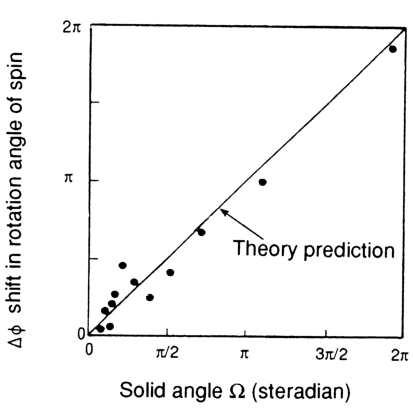
\includegraphics[width=0.6\textwidth]{Figures/BerryPhase.pdf}
\end{center}
\end{document}





































